% Created by tikzDevice version 0.7.0 on 2014-10-24 15:37:23
% !TEX encoding = UTF-8 Unicode
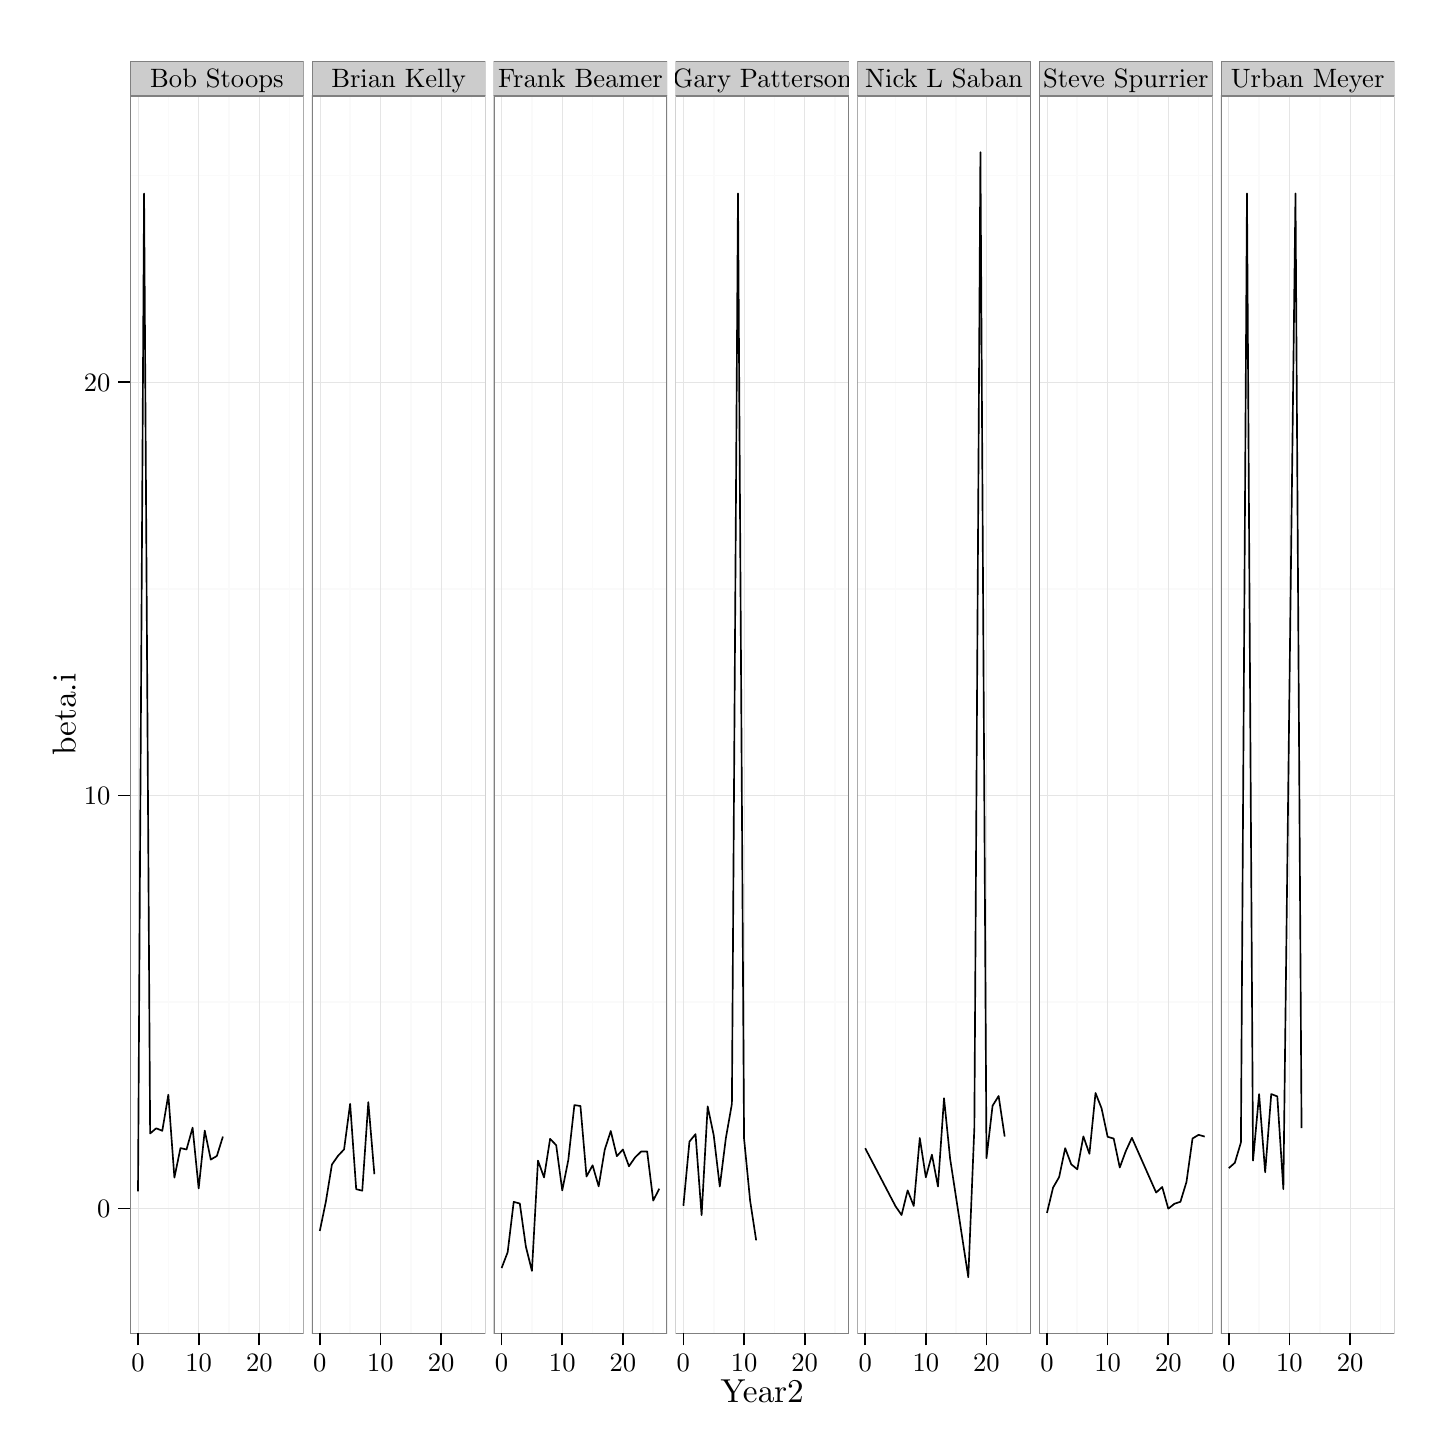
\begin{tikzpicture}[x=1pt,y=1pt]
\definecolor[named]{fillColor}{rgb}{1.00,1.00,1.00}
\path[use as bounding box,fill=fillColor,fill opacity=0.00] (0,0) rectangle (505.89,505.89);
\begin{scope}
\path[clip] (  0.00,  0.00) rectangle (505.89,505.89);
\definecolor[named]{drawColor}{rgb}{1.00,1.00,1.00}
\definecolor[named]{fillColor}{rgb}{1.00,1.00,1.00}

\path[draw=drawColor,line width= 0.6pt,line join=round,line cap=round,fill=fillColor] (  0.00,  0.00) rectangle (505.89,505.89);
\end{scope}
\begin{scope}
\path[clip] ( 37.02,481.21) rectangle ( 99.70,493.85);
\definecolor[named]{drawColor}{rgb}{0.50,0.50,0.50}
\definecolor[named]{fillColor}{rgb}{0.80,0.80,0.80}

\path[draw=drawColor,line width= 0.2pt,line join=round,line cap=round,fill=fillColor] ( 37.02,481.21) rectangle ( 99.70,493.85);
\definecolor[named]{drawColor}{rgb}{0.00,0.00,0.00}

\node[text=drawColor,anchor=base,inner sep=0pt, outer sep=0pt, scale=  0.96] at ( 68.36,484.22) {Bob Stoops};
\end{scope}
\begin{scope}
\path[clip] (102.71,481.21) rectangle (165.39,493.85);
\definecolor[named]{drawColor}{rgb}{0.50,0.50,0.50}
\definecolor[named]{fillColor}{rgb}{0.80,0.80,0.80}

\path[draw=drawColor,line width= 0.2pt,line join=round,line cap=round,fill=fillColor] (102.71,481.21) rectangle (165.39,493.85);
\definecolor[named]{drawColor}{rgb}{0.00,0.00,0.00}

\node[text=drawColor,anchor=base,inner sep=0pt, outer sep=0pt, scale=  0.96] at (134.05,484.22) {Brian Kelly};
\end{scope}
\begin{scope}
\path[clip] (168.40,481.21) rectangle (231.08,493.85);
\definecolor[named]{drawColor}{rgb}{0.50,0.50,0.50}
\definecolor[named]{fillColor}{rgb}{0.80,0.80,0.80}

\path[draw=drawColor,line width= 0.2pt,line join=round,line cap=round,fill=fillColor] (168.40,481.21) rectangle (231.08,493.85);
\definecolor[named]{drawColor}{rgb}{0.00,0.00,0.00}

\node[text=drawColor,anchor=base,inner sep=0pt, outer sep=0pt, scale=  0.96] at (199.74,484.22) {Frank Beamer};
\end{scope}
\begin{scope}
\path[clip] (234.09,481.21) rectangle (296.77,493.85);
\definecolor[named]{drawColor}{rgb}{0.50,0.50,0.50}
\definecolor[named]{fillColor}{rgb}{0.80,0.80,0.80}

\path[draw=drawColor,line width= 0.2pt,line join=round,line cap=round,fill=fillColor] (234.09,481.21) rectangle (296.77,493.85);
\definecolor[named]{drawColor}{rgb}{0.00,0.00,0.00}

\node[text=drawColor,anchor=base,inner sep=0pt, outer sep=0pt, scale=  0.96] at (265.43,484.22) {Gary Patterson};
\end{scope}
\begin{scope}
\path[clip] (299.78,481.21) rectangle (362.46,493.85);
\definecolor[named]{drawColor}{rgb}{0.50,0.50,0.50}
\definecolor[named]{fillColor}{rgb}{0.80,0.80,0.80}

\path[draw=drawColor,line width= 0.2pt,line join=round,line cap=round,fill=fillColor] (299.78,481.21) rectangle (362.46,493.85);
\definecolor[named]{drawColor}{rgb}{0.00,0.00,0.00}

\node[text=drawColor,anchor=base,inner sep=0pt, outer sep=0pt, scale=  0.96] at (331.12,484.22) {Nick L Saban};
\end{scope}
\begin{scope}
\path[clip] (365.47,481.21) rectangle (428.15,493.85);
\definecolor[named]{drawColor}{rgb}{0.50,0.50,0.50}
\definecolor[named]{fillColor}{rgb}{0.80,0.80,0.80}

\path[draw=drawColor,line width= 0.2pt,line join=round,line cap=round,fill=fillColor] (365.47,481.21) rectangle (428.15,493.85);
\definecolor[named]{drawColor}{rgb}{0.00,0.00,0.00}

\node[text=drawColor,anchor=base,inner sep=0pt, outer sep=0pt, scale=  0.96] at (396.81,484.22) {Steve Spurrier};
\end{scope}
\begin{scope}
\path[clip] (431.17,481.21) rectangle (493.85,493.85);
\definecolor[named]{drawColor}{rgb}{0.50,0.50,0.50}
\definecolor[named]{fillColor}{rgb}{0.80,0.80,0.80}

\path[draw=drawColor,line width= 0.2pt,line join=round,line cap=round,fill=fillColor] (431.17,481.21) rectangle (493.85,493.85);
\definecolor[named]{drawColor}{rgb}{0.00,0.00,0.00}

\node[text=drawColor,anchor=base,inner sep=0pt, outer sep=0pt, scale=  0.96] at (462.51,484.22) {Urban Meyer};
\end{scope}
\begin{scope}
\path[clip] ( 37.02, 34.03) rectangle ( 99.70,481.21);
\definecolor[named]{fillColor}{rgb}{1.00,1.00,1.00}

\path[fill=fillColor] ( 37.02, 34.03) rectangle ( 99.70,481.21);
\definecolor[named]{drawColor}{rgb}{0.98,0.98,0.98}

\path[draw=drawColor,line width= 0.6pt,line join=round] ( 37.02,153.83) --
	( 99.70,153.83);

\path[draw=drawColor,line width= 0.6pt,line join=round] ( 37.02,303.13) --
	( 99.70,303.13);

\path[draw=drawColor,line width= 0.6pt,line join=round] ( 37.02,452.43) --
	( 99.70,452.43);

\path[draw=drawColor,line width= 0.6pt,line join=round] ( 50.83, 34.03) --
	( 50.83,481.21);

\path[draw=drawColor,line width= 0.6pt,line join=round] ( 72.74, 34.03) --
	( 72.74,481.21);

\path[draw=drawColor,line width= 0.6pt,line join=round] ( 94.66, 34.03) --
	( 94.66,481.21);
\definecolor[named]{drawColor}{rgb}{0.90,0.90,0.90}

\path[draw=drawColor,line width= 0.2pt,line join=round] ( 37.02, 79.18) --
	( 99.70, 79.18);

\path[draw=drawColor,line width= 0.2pt,line join=round] ( 37.02,228.48) --
	( 99.70,228.48);

\path[draw=drawColor,line width= 0.2pt,line join=round] ( 37.02,377.78) --
	( 99.70,377.78);

\path[draw=drawColor,line width= 0.2pt,line join=round] ( 39.87, 34.03) --
	( 39.87,481.21);

\path[draw=drawColor,line width= 0.2pt,line join=round] ( 61.79, 34.03) --
	( 61.79,481.21);

\path[draw=drawColor,line width= 0.2pt,line join=round] ( 83.70, 34.03) --
	( 83.70,481.21);
\definecolor[named]{drawColor}{rgb}{0.00,0.00,0.00}

\path[draw=drawColor,line width= 0.6pt,line join=round] ( 39.87, 85.37) --
	( 42.06,445.95) --
	( 44.25,106.31) --
	( 46.44,108.18) --
	( 48.64,107.28) --
	( 50.83,120.31) --
	( 53.02, 90.36) --
	( 55.21,101.03) --
	( 57.40,100.52) --
	( 59.59,108.39) --
	( 61.79, 86.45) --
	( 63.98,107.33) --
	( 66.17, 96.88) --
	( 68.36, 98.17) --
	( 70.55,105.19);
\definecolor[named]{drawColor}{rgb}{0.50,0.50,0.50}

\path[draw=drawColor,line width= 0.6pt,line join=round,line cap=round] ( 37.02, 34.03) rectangle ( 99.70,481.21);
\end{scope}
\begin{scope}
\path[clip] (102.71, 34.03) rectangle (165.39,481.21);
\definecolor[named]{fillColor}{rgb}{1.00,1.00,1.00}

\path[fill=fillColor] (102.71, 34.03) rectangle (165.39,481.21);
\definecolor[named]{drawColor}{rgb}{0.98,0.98,0.98}

\path[draw=drawColor,line width= 0.6pt,line join=round] (102.71,153.83) --
	(165.39,153.83);

\path[draw=drawColor,line width= 0.6pt,line join=round] (102.71,303.13) --
	(165.39,303.13);

\path[draw=drawColor,line width= 0.6pt,line join=round] (102.71,452.43) --
	(165.39,452.43);

\path[draw=drawColor,line width= 0.6pt,line join=round] (116.52, 34.03) --
	(116.52,481.21);

\path[draw=drawColor,line width= 0.6pt,line join=round] (138.43, 34.03) --
	(138.43,481.21);

\path[draw=drawColor,line width= 0.6pt,line join=round] (160.35, 34.03) --
	(160.35,481.21);
\definecolor[named]{drawColor}{rgb}{0.90,0.90,0.90}

\path[draw=drawColor,line width= 0.2pt,line join=round] (102.71, 79.18) --
	(165.39, 79.18);

\path[draw=drawColor,line width= 0.2pt,line join=round] (102.71,228.48) --
	(165.39,228.48);

\path[draw=drawColor,line width= 0.2pt,line join=round] (102.71,377.78) --
	(165.39,377.78);

\path[draw=drawColor,line width= 0.2pt,line join=round] (105.56, 34.03) --
	(105.56,481.21);

\path[draw=drawColor,line width= 0.2pt,line join=round] (127.48, 34.03) --
	(127.48,481.21);

\path[draw=drawColor,line width= 0.2pt,line join=round] (149.39, 34.03) --
	(149.39,481.21);
\definecolor[named]{drawColor}{rgb}{0.00,0.00,0.00}

\path[draw=drawColor,line width= 0.6pt,line join=round] (105.56, 71.09) --
	(107.75, 81.68) --
	(109.94, 95.09) --
	(112.14, 98.23) --
	(114.33,100.56) --
	(116.52,117.02) --
	(118.71, 86.18) --
	(120.90, 85.63) --
	(123.09,117.63) --
	(125.28, 91.58);
\definecolor[named]{drawColor}{rgb}{0.50,0.50,0.50}

\path[draw=drawColor,line width= 0.6pt,line join=round,line cap=round] (102.71, 34.03) rectangle (165.39,481.21);
\end{scope}
\begin{scope}
\path[clip] (168.40, 34.03) rectangle (231.08,481.21);
\definecolor[named]{fillColor}{rgb}{1.00,1.00,1.00}

\path[fill=fillColor] (168.40, 34.03) rectangle (231.08,481.21);
\definecolor[named]{drawColor}{rgb}{0.98,0.98,0.98}

\path[draw=drawColor,line width= 0.6pt,line join=round] (168.40,153.83) --
	(231.08,153.83);

\path[draw=drawColor,line width= 0.6pt,line join=round] (168.40,303.13) --
	(231.08,303.13);

\path[draw=drawColor,line width= 0.6pt,line join=round] (168.40,452.43) --
	(231.08,452.43);

\path[draw=drawColor,line width= 0.6pt,line join=round] (182.21, 34.03) --
	(182.21,481.21);

\path[draw=drawColor,line width= 0.6pt,line join=round] (204.13, 34.03) --
	(204.13,481.21);

\path[draw=drawColor,line width= 0.6pt,line join=round] (226.04, 34.03) --
	(226.04,481.21);
\definecolor[named]{drawColor}{rgb}{0.90,0.90,0.90}

\path[draw=drawColor,line width= 0.2pt,line join=round] (168.40, 79.18) --
	(231.08, 79.18);

\path[draw=drawColor,line width= 0.2pt,line join=round] (168.40,228.48) --
	(231.08,228.48);

\path[draw=drawColor,line width= 0.2pt,line join=round] (168.40,377.78) --
	(231.08,377.78);

\path[draw=drawColor,line width= 0.2pt,line join=round] (171.25, 34.03) --
	(171.25,481.21);

\path[draw=drawColor,line width= 0.2pt,line join=round] (193.17, 34.03) --
	(193.17,481.21);

\path[draw=drawColor,line width= 0.2pt,line join=round] (215.08, 34.03) --
	(215.08,481.21);
\definecolor[named]{drawColor}{rgb}{0.00,0.00,0.00}

\path[draw=drawColor,line width= 0.6pt,line join=round] (171.25, 57.67) --
	(173.44, 63.39) --
	(175.63, 81.59) --
	(177.83, 81.00) --
	(180.02, 65.44) --
	(182.21, 56.64) --
	(184.40, 96.49) --
	(186.59, 90.42) --
	(188.78,104.38) --
	(190.98,102.07) --
	(193.17, 85.74) --
	(195.36, 96.76) --
	(197.55,116.56) --
	(199.74,116.24) --
	(201.93, 90.75) --
	(204.13, 94.80) --
	(206.32, 87.20) --
	(208.51,100.41) --
	(210.70,107.20) --
	(212.89, 98.10) --
	(215.08,100.52) --
	(217.27, 94.46) --
	(219.47, 97.64) --
	(221.66, 99.77) --
	(223.85, 99.81) --
	(226.04, 82.06) --
	(228.23, 86.36);
\definecolor[named]{drawColor}{rgb}{0.50,0.50,0.50}

\path[draw=drawColor,line width= 0.6pt,line join=round,line cap=round] (168.40, 34.03) rectangle (231.08,481.21);
\end{scope}
\begin{scope}
\path[clip] (234.09, 34.03) rectangle (296.77,481.21);
\definecolor[named]{fillColor}{rgb}{1.00,1.00,1.00}

\path[fill=fillColor] (234.09, 34.03) rectangle (296.77,481.21);
\definecolor[named]{drawColor}{rgb}{0.98,0.98,0.98}

\path[draw=drawColor,line width= 0.6pt,line join=round] (234.09,153.83) --
	(296.77,153.83);

\path[draw=drawColor,line width= 0.6pt,line join=round] (234.09,303.13) --
	(296.77,303.13);

\path[draw=drawColor,line width= 0.6pt,line join=round] (234.09,452.43) --
	(296.77,452.43);

\path[draw=drawColor,line width= 0.6pt,line join=round] (247.90, 34.03) --
	(247.90,481.21);

\path[draw=drawColor,line width= 0.6pt,line join=round] (269.82, 34.03) --
	(269.82,481.21);

\path[draw=drawColor,line width= 0.6pt,line join=round] (291.73, 34.03) --
	(291.73,481.21);
\definecolor[named]{drawColor}{rgb}{0.90,0.90,0.90}

\path[draw=drawColor,line width= 0.2pt,line join=round] (234.09, 79.18) --
	(296.77, 79.18);

\path[draw=drawColor,line width= 0.2pt,line join=round] (234.09,228.48) --
	(296.77,228.48);

\path[draw=drawColor,line width= 0.2pt,line join=round] (234.09,377.78) --
	(296.77,377.78);

\path[draw=drawColor,line width= 0.2pt,line join=round] (236.94, 34.03) --
	(236.94,481.21);

\path[draw=drawColor,line width= 0.2pt,line join=round] (258.86, 34.03) --
	(258.86,481.21);

\path[draw=drawColor,line width= 0.2pt,line join=round] (280.77, 34.03) --
	(280.77,481.21);
\definecolor[named]{drawColor}{rgb}{0.00,0.00,0.00}

\path[draw=drawColor,line width= 0.6pt,line join=round] (236.94, 80.18) --
	(239.13,103.38) --
	(241.33,106.08) --
	(243.52, 76.77) --
	(245.71,116.11) --
	(247.90,105.66) --
	(250.09, 87.13) --
	(252.28,104.58) --
	(254.47,117.02) --
	(256.67,445.95) --
	(258.86,104.51) --
	(261.05, 82.06) --
	(263.24, 67.69);
\definecolor[named]{drawColor}{rgb}{0.50,0.50,0.50}

\path[draw=drawColor,line width= 0.6pt,line join=round,line cap=round] (234.09, 34.03) rectangle (296.77,481.21);
\end{scope}
\begin{scope}
\path[clip] (299.78, 34.03) rectangle (362.46,481.21);
\definecolor[named]{fillColor}{rgb}{1.00,1.00,1.00}

\path[fill=fillColor] (299.78, 34.03) rectangle (362.46,481.21);
\definecolor[named]{drawColor}{rgb}{0.98,0.98,0.98}

\path[draw=drawColor,line width= 0.6pt,line join=round] (299.78,153.83) --
	(362.46,153.83);

\path[draw=drawColor,line width= 0.6pt,line join=round] (299.78,303.13) --
	(362.46,303.13);

\path[draw=drawColor,line width= 0.6pt,line join=round] (299.78,452.43) --
	(362.46,452.43);

\path[draw=drawColor,line width= 0.6pt,line join=round] (313.59, 34.03) --
	(313.59,481.21);

\path[draw=drawColor,line width= 0.6pt,line join=round] (335.51, 34.03) --
	(335.51,481.21);

\path[draw=drawColor,line width= 0.6pt,line join=round] (357.42, 34.03) --
	(357.42,481.21);
\definecolor[named]{drawColor}{rgb}{0.90,0.90,0.90}

\path[draw=drawColor,line width= 0.2pt,line join=round] (299.78, 79.18) --
	(362.46, 79.18);

\path[draw=drawColor,line width= 0.2pt,line join=round] (299.78,228.48) --
	(362.46,228.48);

\path[draw=drawColor,line width= 0.2pt,line join=round] (299.78,377.78) --
	(362.46,377.78);

\path[draw=drawColor,line width= 0.2pt,line join=round] (302.63, 34.03) --
	(302.63,481.21);

\path[draw=drawColor,line width= 0.2pt,line join=round] (324.55, 34.03) --
	(324.55,481.21);

\path[draw=drawColor,line width= 0.2pt,line join=round] (346.46, 34.03) --
	(346.46,481.21);
\definecolor[named]{drawColor}{rgb}{0.00,0.00,0.00}

\path[draw=drawColor,line width= 0.6pt,line join=round] (302.63,100.98) --
	(313.59, 80.02) --
	(315.78, 76.84) --
	(317.97, 85.74) --
	(320.17, 80.12) --
	(322.36,104.67) --
	(324.55, 90.46) --
	(326.74, 98.66) --
	(328.93, 87.15) --
	(331.12,119.06) --
	(333.32, 97.23) --
	(339.89, 54.36) --
	(342.08,108.40) --
	(344.27,460.88) --
	(346.46, 97.39) --
	(348.66,116.32) --
	(350.85,119.85) --
	(353.04,105.19);
\definecolor[named]{drawColor}{rgb}{0.50,0.50,0.50}

\path[draw=drawColor,line width= 0.6pt,line join=round,line cap=round] (299.78, 34.03) rectangle (362.46,481.21);
\end{scope}
\begin{scope}
\path[clip] (365.47, 34.03) rectangle (428.15,481.21);
\definecolor[named]{fillColor}{rgb}{1.00,1.00,1.00}

\path[fill=fillColor] (365.47, 34.03) rectangle (428.15,481.21);
\definecolor[named]{drawColor}{rgb}{0.98,0.98,0.98}

\path[draw=drawColor,line width= 0.6pt,line join=round] (365.47,153.83) --
	(428.15,153.83);

\path[draw=drawColor,line width= 0.6pt,line join=round] (365.47,303.13) --
	(428.15,303.13);

\path[draw=drawColor,line width= 0.6pt,line join=round] (365.47,452.43) --
	(428.15,452.43);

\path[draw=drawColor,line width= 0.6pt,line join=round] (379.28, 34.03) --
	(379.28,481.21);

\path[draw=drawColor,line width= 0.6pt,line join=round] (401.20, 34.03) --
	(401.20,481.21);

\path[draw=drawColor,line width= 0.6pt,line join=round] (423.11, 34.03) --
	(423.11,481.21);
\definecolor[named]{drawColor}{rgb}{0.90,0.90,0.90}

\path[draw=drawColor,line width= 0.2pt,line join=round] (365.47, 79.18) --
	(428.15, 79.18);

\path[draw=drawColor,line width= 0.2pt,line join=round] (365.47,228.48) --
	(428.15,228.48);

\path[draw=drawColor,line width= 0.2pt,line join=round] (365.47,377.78) --
	(428.15,377.78);

\path[draw=drawColor,line width= 0.2pt,line join=round] (368.32, 34.03) --
	(368.32,481.21);

\path[draw=drawColor,line width= 0.2pt,line join=round] (390.24, 34.03) --
	(390.24,481.21);

\path[draw=drawColor,line width= 0.2pt,line join=round] (412.16, 34.03) --
	(412.16,481.21);
\definecolor[named]{drawColor}{rgb}{0.00,0.00,0.00}

\path[draw=drawColor,line width= 0.6pt,line join=round] (368.32, 77.60) --
	(370.52, 86.74) --
	(372.71, 90.54) --
	(374.90,100.99) --
	(377.09, 95.17) --
	(379.28, 93.36) --
	(381.47,105.26) --
	(383.66, 98.95) --
	(385.86,120.93) --
	(388.05,115.39) --
	(390.24,105.10) --
	(392.43,104.47) --
	(394.62, 94.01) --
	(396.81, 99.96) --
	(399.01,104.73) --
	(407.77, 84.96) --
	(409.96, 86.97) --
	(412.16, 79.13) --
	(414.35, 80.89) --
	(416.54, 81.62) --
	(418.73, 88.79) --
	(420.92,104.51) --
	(423.11,105.81) --
	(425.31,105.19);
\definecolor[named]{drawColor}{rgb}{0.50,0.50,0.50}

\path[draw=drawColor,line width= 0.6pt,line join=round,line cap=round] (365.47, 34.03) rectangle (428.15,481.21);
\end{scope}
\begin{scope}
\path[clip] (431.17, 34.03) rectangle (493.85,481.21);
\definecolor[named]{fillColor}{rgb}{1.00,1.00,1.00}

\path[fill=fillColor] (431.17, 34.03) rectangle (493.85,481.21);
\definecolor[named]{drawColor}{rgb}{0.98,0.98,0.98}

\path[draw=drawColor,line width= 0.6pt,line join=round] (431.17,153.83) --
	(493.85,153.83);

\path[draw=drawColor,line width= 0.6pt,line join=round] (431.17,303.13) --
	(493.85,303.13);

\path[draw=drawColor,line width= 0.6pt,line join=round] (431.17,452.43) --
	(493.85,452.43);

\path[draw=drawColor,line width= 0.6pt,line join=round] (444.97, 34.03) --
	(444.97,481.21);

\path[draw=drawColor,line width= 0.6pt,line join=round] (466.89, 34.03) --
	(466.89,481.21);

\path[draw=drawColor,line width= 0.6pt,line join=round] (488.80, 34.03) --
	(488.80,481.21);
\definecolor[named]{drawColor}{rgb}{0.90,0.90,0.90}

\path[draw=drawColor,line width= 0.2pt,line join=round] (431.17, 79.18) --
	(493.85, 79.18);

\path[draw=drawColor,line width= 0.2pt,line join=round] (431.17,228.48) --
	(493.85,228.48);

\path[draw=drawColor,line width= 0.2pt,line join=round] (431.17,377.78) --
	(493.85,377.78);

\path[draw=drawColor,line width= 0.2pt,line join=round] (434.01, 34.03) --
	(434.01,481.21);

\path[draw=drawColor,line width= 0.2pt,line join=round] (455.93, 34.03) --
	(455.93,481.21);

\path[draw=drawColor,line width= 0.2pt,line join=round] (477.85, 34.03) --
	(477.85,481.21);
\definecolor[named]{drawColor}{rgb}{0.00,0.00,0.00}

\path[draw=drawColor,line width= 0.6pt,line join=round] (434.01, 93.77) --
	(436.21, 95.72) --
	(438.40,103.05) --
	(440.59,445.95) --
	(442.78, 96.50) --
	(444.97,120.53) --
	(447.16, 92.29) --
	(449.36,120.55) --
	(451.55,119.70) --
	(453.74, 86.18) --
	(458.12,445.95) --
	(460.31,108.25);
\definecolor[named]{drawColor}{rgb}{0.50,0.50,0.50}

\path[draw=drawColor,line width= 0.6pt,line join=round,line cap=round] (431.17, 34.03) rectangle (493.85,481.21);
\end{scope}
\begin{scope}
\path[clip] (  0.00,  0.00) rectangle (505.89,505.89);
\definecolor[named]{drawColor}{rgb}{0.00,0.00,0.00}

\node[text=drawColor,anchor=base east,inner sep=0pt, outer sep=0pt, scale=  0.96] at ( 29.91, 75.88) {0};

\node[text=drawColor,anchor=base east,inner sep=0pt, outer sep=0pt, scale=  0.96] at ( 29.91,225.18) {10};

\node[text=drawColor,anchor=base east,inner sep=0pt, outer sep=0pt, scale=  0.96] at ( 29.91,374.48) {20};
\end{scope}
\begin{scope}
\path[clip] (  0.00,  0.00) rectangle (505.89,505.89);
\definecolor[named]{drawColor}{rgb}{0.00,0.00,0.00}

\path[draw=drawColor,line width= 0.6pt,line join=round] ( 32.75, 79.18) --
	( 37.02, 79.18);

\path[draw=drawColor,line width= 0.6pt,line join=round] ( 32.75,228.48) --
	( 37.02,228.48);

\path[draw=drawColor,line width= 0.6pt,line join=round] ( 32.75,377.78) --
	( 37.02,377.78);
\end{scope}
\begin{scope}
\path[clip] (  0.00,  0.00) rectangle (505.89,505.89);
\definecolor[named]{drawColor}{rgb}{0.00,0.00,0.00}

\path[draw=drawColor,line width= 0.6pt,line join=round] ( 39.87, 29.77) --
	( 39.87, 34.03);

\path[draw=drawColor,line width= 0.6pt,line join=round] ( 61.79, 29.77) --
	( 61.79, 34.03);

\path[draw=drawColor,line width= 0.6pt,line join=round] ( 83.70, 29.77) --
	( 83.70, 34.03);
\end{scope}
\begin{scope}
\path[clip] (  0.00,  0.00) rectangle (505.89,505.89);
\definecolor[named]{drawColor}{rgb}{0.00,0.00,0.00}

\node[text=drawColor,anchor=base,inner sep=0pt, outer sep=0pt, scale=  0.96] at ( 39.87, 20.31) {0};

\node[text=drawColor,anchor=base,inner sep=0pt, outer sep=0pt, scale=  0.96] at ( 61.79, 20.31) {10};

\node[text=drawColor,anchor=base,inner sep=0pt, outer sep=0pt, scale=  0.96] at ( 83.70, 20.31) {20};
\end{scope}
\begin{scope}
\path[clip] (  0.00,  0.00) rectangle (505.89,505.89);
\definecolor[named]{drawColor}{rgb}{0.00,0.00,0.00}

\path[draw=drawColor,line width= 0.6pt,line join=round] (105.56, 29.77) --
	(105.56, 34.03);

\path[draw=drawColor,line width= 0.6pt,line join=round] (127.48, 29.77) --
	(127.48, 34.03);

\path[draw=drawColor,line width= 0.6pt,line join=round] (149.39, 29.77) --
	(149.39, 34.03);
\end{scope}
\begin{scope}
\path[clip] (  0.00,  0.00) rectangle (505.89,505.89);
\definecolor[named]{drawColor}{rgb}{0.00,0.00,0.00}

\node[text=drawColor,anchor=base,inner sep=0pt, outer sep=0pt, scale=  0.96] at (105.56, 20.31) {0};

\node[text=drawColor,anchor=base,inner sep=0pt, outer sep=0pt, scale=  0.96] at (127.48, 20.31) {10};

\node[text=drawColor,anchor=base,inner sep=0pt, outer sep=0pt, scale=  0.96] at (149.39, 20.31) {20};
\end{scope}
\begin{scope}
\path[clip] (  0.00,  0.00) rectangle (505.89,505.89);
\definecolor[named]{drawColor}{rgb}{0.00,0.00,0.00}

\path[draw=drawColor,line width= 0.6pt,line join=round] (171.25, 29.77) --
	(171.25, 34.03);

\path[draw=drawColor,line width= 0.6pt,line join=round] (193.17, 29.77) --
	(193.17, 34.03);

\path[draw=drawColor,line width= 0.6pt,line join=round] (215.08, 29.77) --
	(215.08, 34.03);
\end{scope}
\begin{scope}
\path[clip] (  0.00,  0.00) rectangle (505.89,505.89);
\definecolor[named]{drawColor}{rgb}{0.00,0.00,0.00}

\node[text=drawColor,anchor=base,inner sep=0pt, outer sep=0pt, scale=  0.96] at (171.25, 20.31) {0};

\node[text=drawColor,anchor=base,inner sep=0pt, outer sep=0pt, scale=  0.96] at (193.17, 20.31) {10};

\node[text=drawColor,anchor=base,inner sep=0pt, outer sep=0pt, scale=  0.96] at (215.08, 20.31) {20};
\end{scope}
\begin{scope}
\path[clip] (  0.00,  0.00) rectangle (505.89,505.89);
\definecolor[named]{drawColor}{rgb}{0.00,0.00,0.00}

\path[draw=drawColor,line width= 0.6pt,line join=round] (236.94, 29.77) --
	(236.94, 34.03);

\path[draw=drawColor,line width= 0.6pt,line join=round] (258.86, 29.77) --
	(258.86, 34.03);

\path[draw=drawColor,line width= 0.6pt,line join=round] (280.77, 29.77) --
	(280.77, 34.03);
\end{scope}
\begin{scope}
\path[clip] (  0.00,  0.00) rectangle (505.89,505.89);
\definecolor[named]{drawColor}{rgb}{0.00,0.00,0.00}

\node[text=drawColor,anchor=base,inner sep=0pt, outer sep=0pt, scale=  0.96] at (236.94, 20.31) {0};

\node[text=drawColor,anchor=base,inner sep=0pt, outer sep=0pt, scale=  0.96] at (258.86, 20.31) {10};

\node[text=drawColor,anchor=base,inner sep=0pt, outer sep=0pt, scale=  0.96] at (280.77, 20.31) {20};
\end{scope}
\begin{scope}
\path[clip] (  0.00,  0.00) rectangle (505.89,505.89);
\definecolor[named]{drawColor}{rgb}{0.00,0.00,0.00}

\path[draw=drawColor,line width= 0.6pt,line join=round] (302.63, 29.77) --
	(302.63, 34.03);

\path[draw=drawColor,line width= 0.6pt,line join=round] (324.55, 29.77) --
	(324.55, 34.03);

\path[draw=drawColor,line width= 0.6pt,line join=round] (346.46, 29.77) --
	(346.46, 34.03);
\end{scope}
\begin{scope}
\path[clip] (  0.00,  0.00) rectangle (505.89,505.89);
\definecolor[named]{drawColor}{rgb}{0.00,0.00,0.00}

\node[text=drawColor,anchor=base,inner sep=0pt, outer sep=0pt, scale=  0.96] at (302.63, 20.31) {0};

\node[text=drawColor,anchor=base,inner sep=0pt, outer sep=0pt, scale=  0.96] at (324.55, 20.31) {10};

\node[text=drawColor,anchor=base,inner sep=0pt, outer sep=0pt, scale=  0.96] at (346.46, 20.31) {20};
\end{scope}
\begin{scope}
\path[clip] (  0.00,  0.00) rectangle (505.89,505.89);
\definecolor[named]{drawColor}{rgb}{0.00,0.00,0.00}

\path[draw=drawColor,line width= 0.6pt,line join=round] (368.32, 29.77) --
	(368.32, 34.03);

\path[draw=drawColor,line width= 0.6pt,line join=round] (390.24, 29.77) --
	(390.24, 34.03);

\path[draw=drawColor,line width= 0.6pt,line join=round] (412.16, 29.77) --
	(412.16, 34.03);
\end{scope}
\begin{scope}
\path[clip] (  0.00,  0.00) rectangle (505.89,505.89);
\definecolor[named]{drawColor}{rgb}{0.00,0.00,0.00}

\node[text=drawColor,anchor=base,inner sep=0pt, outer sep=0pt, scale=  0.96] at (368.32, 20.31) {0};

\node[text=drawColor,anchor=base,inner sep=0pt, outer sep=0pt, scale=  0.96] at (390.24, 20.31) {10};

\node[text=drawColor,anchor=base,inner sep=0pt, outer sep=0pt, scale=  0.96] at (412.16, 20.31) {20};
\end{scope}
\begin{scope}
\path[clip] (  0.00,  0.00) rectangle (505.89,505.89);
\definecolor[named]{drawColor}{rgb}{0.00,0.00,0.00}

\path[draw=drawColor,line width= 0.6pt,line join=round] (434.01, 29.77) --
	(434.01, 34.03);

\path[draw=drawColor,line width= 0.6pt,line join=round] (455.93, 29.77) --
	(455.93, 34.03);

\path[draw=drawColor,line width= 0.6pt,line join=round] (477.85, 29.77) --
	(477.85, 34.03);
\end{scope}
\begin{scope}
\path[clip] (  0.00,  0.00) rectangle (505.89,505.89);
\definecolor[named]{drawColor}{rgb}{0.00,0.00,0.00}

\node[text=drawColor,anchor=base,inner sep=0pt, outer sep=0pt, scale=  0.96] at (434.01, 20.31) {0};

\node[text=drawColor,anchor=base,inner sep=0pt, outer sep=0pt, scale=  0.96] at (455.93, 20.31) {10};

\node[text=drawColor,anchor=base,inner sep=0pt, outer sep=0pt, scale=  0.96] at (477.85, 20.31) {20};
\end{scope}
\begin{scope}
\path[clip] (  0.00,  0.00) rectangle (505.89,505.89);
\definecolor[named]{drawColor}{rgb}{0.00,0.00,0.00}

\node[text=drawColor,anchor=base,inner sep=0pt, outer sep=0pt, scale=  1.20] at (265.43,  9.03) {Year2};
\end{scope}
\begin{scope}
\path[clip] (  0.00,  0.00) rectangle (505.89,505.89);
\definecolor[named]{drawColor}{rgb}{0.00,0.00,0.00}

\node[text=drawColor,rotate= 90.00,anchor=base,inner sep=0pt, outer sep=0pt, scale=  1.20] at ( 17.30,257.62) {beta.i};
\end{scope}
\end{tikzpicture}
